\documentclass{prrcs}
\usepackage{parskip}
\usepackage{overpic}
\usepackage[font=small]{caption}
\usepackage{subcaption}
\graphicspath{{../images/}}
\newcommand{\cmmnt}[1]{}

%====================================================

\begin{document}

\title{%
    \vspace{-0.75cm}%
    Holistic Dashboard of Software\\Development Work-Time \& Practices%
}

\author{%
    \vspace{-0.5cm}%
    Inesh Bose \& Dr. Tim Storer (University of Glasgow)%
}

\date{}

\maketitle

%====================================================
\section*{Abstract}

Ensuring success \& efficient development of software heavily relies on Developer Experience (DX). Products that provide a good user experience attract more customers who wish to not increase any frustrations while using their services; similarly, a software project with good developer experience \& relations would enable the individuals to be more productive and motivated to continue working with the aim of quality output. Many projects fail when there is a lack of consideration for good DX and the project members are frustrated as they continue to work, without knowing other better tools available, increasing technical debt, with a tight budget and a nearing deadline; much of this can be mitigated with appropriate estimations of their task by realising their knowledge and efforts taken in making changes on the code repository. This project aims to research Developer Experience, task-effort estimations \& the relationship between them, providing a solution through the means of a centralised modular dashboard, showing visualisations of their development activity, that will be evaluated with developers and their teams in real-life scenarios as they work on their important software projects over a period of time.

%====================================================
\section{Background}

% Introduce the proposal topic and explain its academic, industrial, policy, societal, or other relevant context. Indicate who might benefit from the research, and how.

% Explain where this work fits in the current portfolio of EPSRC-funded research and how it relates to past and current work in the UK and abroad.

There is significant importance given to a good User Experience (UX) in a product - which is reasonable - however, there is another area that requires equal importance which is Developer Experience (DX); it pertains to the humans working on a project as software developers -- but project frustration is widespread in any industry. A person's mood affects their problem-solving skills and productivity \cite{amabileProgressPrincipleUsing2011,graziotinFeelingsMatterCorrelation2015,meyerSoftwareDevelopersPerceptions2014,mullerStuckFrustratedFlow2015}, and in software development, this influences performance on certain tasks such as implementing, testing and debugging \cite{khanMoodsAffectProgrammers2011}. Companies and organisations take measures on helping their staff destress and have a better experience, but this may not be effective or formalised. Working on software is different to other industries as it requires a level of mental cognition in unique, non-repeating processes \cite{trendowiczChapterFactorsInfluencing2009,abdel-hamidSlipperyPathProductivity1996,briand2002software,kemererEmpiricalValidationSoftware1987}. It must be realised that \textbf{humans are the most important aspect of software engineering \cite{martinAgileSoftwareDevelopment2003}}, and we plan to address the common obstacles and frustrations that they face as they apply various disciplines to deliver reliable, efficient and high-quality products \cite{sommervilleSoftwareEngineering1992}.

Given our experience working on software projects with different team structures, we realise the diversity of developers and software processes. Starting from choosing \& setting up the appropriate tools for the project from an enormous range of options, like 420K projects with more than 4M releases on PyPI \cite{PyPIPythonPackagea} and more than 1M on npm.js \cite{NpmBlogArchive}, there is scope to mitigate developer frustration with the right tools as the foundations of their product \& development environment that developers and their teams build upon; however, continuing development without the right foundation tends to increase technical debt without developers realising. Moreover, in teams, discussing tools \& tasks may be challenging as the team members may individually have different 1) experiences - such as previously being exposed to projects using different technologies or having their first project as a novice graduate; 2) priorities - such as being motivated to deliver better quality solutions or completing the task as quickly as possible; and 3) beliefs - based on their good and bad experiences, they may judge the suitability of strategies or solutions differently. At university, these differences are commonly experienced within student teams \cite{waiteStudentCultureVs2004} that also look to develop projects for their courses with minimum efforts to get a passing grade \cite{marzoloExtremeDevelopmentMeans2021}.

Given the differences of human factors in software, one of the fundamental steps of software development is effort estimation, and it is necessary that realistic and accurate numbers are used to encourage success and better health of the project. When the target estimation is not met, either the customers provided a larger budget, or more commonly \cite{molokkenReviewSoftwareSurveys2003,jorgensenBetterSureSafe2004}, the developers were over-optimistic and get frustrated at spending more effort than anticipated also causing a lower budget for other tasks and/or implement non-ideal, quick solutions, therefore, affecting the state of the project. Expert estimation using approaches like Planning Poker \cite{grenningPlanningPokerHow2002} in groups or word-breakdown structure \cite{cicalaDevelopingWorkBreakdown2020} is the dominant strategy \cite{jorgensenReviewStudiesExpert2004}, but educating an estimate requires knowledge of resources.

% ensuring that the developers' time to the project is considered with regards to their subjective journey that may include non-apparent tasks such as environment configuration, forum discussions and testing
The developers and their time being the crucial resource in a process, it is important to realise productivity. Studies have shown that productivity cannot be measured accurately by technical metrics (such as lines of code per work-month \cite{barry1981software,conteSoftwareEngineeringMetrics1986}\cmmnt{{,jonesProgrammingProductivity1985,devanbuAnalyticalEmpiricalEvaluation1996,walstonMethodProgrammingMeasurement1977}}, function points \cite{albrecht1979measuring,computerstaffSoftwareMetricsGood1994}, and change requests fulfilled \cite{cataldoSociotechnicalCongruenceFramework2008,millerHowWasYour2021}) and is highly subjective depending on developers, while organisations tend to continue measuring this way \cite{careyImpactCommunicationMode1997,barry1981software,conteSoftwareEngineeringMetrics1986}\cmmnt{,jonesProgrammingProductivity1985,devanbuAnalyticalEmpiricalEvaluation1996,walstonMethodProgrammingMeasurement1977,albrecht1979measuring,computerstaffSoftwareMetricsGood1994,cataldoSociotechnicalCongruenceFramework2008,millerHowWasYour2021}. There are various different areas that a project may be looking for that may not require technical implementation - such as searching \cite{baoTrackingAnalyzingCrossCutting2015}\cmmnt{,simArchetypalSourceCode1998,stoleeSolvingSearchSource2014,sadowskiHowDevelopersSearch2015,bajracharyaMiningSearchTopics2009,bajracharyaAnalyzingMiningCode2012,xia2017developers}, learning \cite{kafer2017best}\cmmnt{,gillProductivityImpactsSoftware1990,deomeloInterpretativeCaseStudies2013,maxwellBenchmarkingSoftwareDevelopmentProductivity2000,oliveiraSoftwareProjectManagers2016,alexanderUsabilityPrintOnline2013,devaney2009impact,payneAnimatedDemonstrationsExploratory1992,mestreStudentPreferenceTutorial2012,baeckerShowingInsteadTelling2002,lloydScreencastTutorialsEnhance2012,vandermeijComparisonPaperbasedVideo2014,begelNoviceSoftwareDevelopers2008,cockburnCostsBenefitsPair2001,murphy2011peer,murphy-hillHowUsersDiscover2015,marzoloExtremeDevelopmentMeans2021,grossmanSurveySoftwareLearnability2009,campbellDesigningRefactoringTools2008,roehm2012professional,murphy2019developers}, investigating and exploring solutions through forums or discussions \cite{roehm2012professional}; software development is not a linear path \cite{abdel-hamidSlipperyPathProductivity1996,briand2002software,kemererEmpiricalValidationSoftware1987}, and we need to provide a way to present the human efforts taken to write each line of code. \textcite{trendowiczChapterFactorsInfluencing2009} lists the human factors influencing productivity based on over a hundred publications along with their experiences involving industrial projects, workshops and surveys on software productivity, eventually learning that productivity of software development processes would depend significantly on the capabilities of the developers along with the tools and methods that they use; \textbf{the first step of quantifying productivity management is selecting the right metrics}. While some services or organisations may internally provide a product to track metrics, a state-of-the-art solution widely adopted by developers is not known to exist.

%====================================================
\section*{Contribution to knowledge}

% Describe how your research would benefit national and international researchers in the field and related disciplines.

% Detail what will be done to ensure that they can benefit, including any opportunities to engage with researchers in other disciplines to broaden the reach of the new knowledge.

The planned contributions of this project, as discussed below, lookout to provide more insight into Developer Experience while hoping to provide benefit to other researchers in the field.

\subsection*{Key Idea}

\textit{"To determine the effect in development practice \& experience presented by a modular dashboard that uncovers their efforts and present metrics of their choice to help correspond future estimation and allocation of efforts \& resources"}

The planned approach involves conducting a survey on the many areas of development processes including learning, communications and structures. Through the courses at the University of Glasgow that require software development, outline requirements \& solutions that may help students in task estimation; the solution can be implemented and evaluated with the same students over the few weeks of the course.

We know that interfaces and visualisations are the core concepts of interaction between humans and computers\footnote{Branch of study is called "\textit{Human-Computer Interaction}"} \cite{liCategorisationVisualisationMethods2016}. The most notable interface that developers - who are also human - use is a form of Integrated Development Environment (IDE) with the main component being the Text Editor in which they provide a low-level form of instructions to the computer - using software development - to allow end-users to interact with their tools using relatively higher-level interfaces.

Software development (ideally) uses version control for the majority of work on the codebase; this helps greatly in monitoring files and keeping track of changes; the most common tool for this is Git \cite{Git,loeligerVersionControlGit2012}. A change (or \textit{"revision"}) is a snapshot of the codebase and is associated with a timestamp, the author and metrics for the change (in terms of additions and deletions, called \textit{"diff")}; this is also called a commit \cite{wingerdPracticalPerforce2005}. These commits, however, are discrete events on the software development timeline and they do not convey the efforts required to make that change -- there are a lot of contexts \& journeys in between the commits and it is useful to capture them. As we have established, since the humans developing software and choosing metrics are important, we want to present the developers with a tool that uncovers developers' efforts and allows them to choose specific, non-generic tools and make judgements on unpacking future tasks. This means we would be iteratively designing \& developing a prototype dashboard, and evaluating its impact on developers by recording effects on estimation and productivity in their project process.

\textbf{Example:} A duo of developers (Alice \& Bob) are working from their garage on a new project that they believe would be ground-breaking and would be open-source at a later stage. They want to ensure they build the project streamlined from the foundation without creating any potential for technical debt. With the current tools and limited resources, they are worried about using their efforts in appropriate areas and not spending any more time than required. Moreover, the project should have no issues in scaling even if it is mostly being implemented by Alice while Bob manages the requirements \& design. Making the codebase open-source means it would be open for contribution - which would be a huge help - but developers may have different understandings and different skillsets; the changes must be objective and consistent. Using our solution, they would be able to monitor, judge and predict areas of the project that need work so that they can avoid technical debt and map appropriate efforts to future tasks.

\subsection*{Beneficiaries}

Researchers in the field of software engineering \& human-computer interaction and software developers in various team structures, globally, would benefit from this project as it aims to contribute to the understanding of Developer Experience (DX) and how a modular dashboard can expose developers' efforts by presenting metrics of their choice that can be used to allocate resources in future tasks. Data visualisation, machine learning, and artificial intelligence research can also benefit from this project as it involves designing a prototype dashboard that can be customised to present relevant metrics based on the developers' preferences, and researchers can learn from the process of designing the dashboard applying the same techniques to develop tools for other domains.

%====================================================
\section*{National importance}

% The purpose of the national importance criterion is to encourage applicants to articulate why it’s important for their research to be supported by the UK taxpayer so that the UK remains internationally competitive.

% The national importance criterion has a number of strands and so applicants should consider why the research might benefit the UK economy; why it may lead to advances in a different academic discipline, or why it’s important that an internationally leading group continues to be supported.

% Explain how the long-term effects of the proposed research may:
% - contribute to the health of other research disciplines, to current or future UK economic success; to the future development of key emerging industries; or address key UK societal challenges
% - meet national strategic needs by establishing or maintaining unique world-leading research activities, including areas of niche capability
% - fit with and complement other research in the UK portfolio, and EPSRC’s portfolio and strategy.

By all means possible, the project is aimed to make the invested resources worthwhile and provide benefits nationally.

\subsection*{Industry}

Countless development tools such as Neovim, GitHub Copilot, and Prisma ORM, unarguably having developers as their target end-users, focus majorly on developer experience and boast unique features that make such tools preferable. The organisations behind such tools also employ individuals for Developer Relations. Given the rise of web development and JavaScript packages \cite{StackOverflowDeveloper,StateJS2021}, there are often discussions about the most preferable front-end framework \cite{UnderstandingClientsideJavaScript2023}, and packages such as Vue\cmmnt{\cite{VueJsProgressive}} and the uprising Svelte\cmmnt{\cite{SvelteCyberneticallyEnhanced}}, that provide the Single-File Component architecture (with more HTML syntax than functional JSX), enable easy learning and faster development hence are incredibly loved by a global community.

With this in mind, this project can provide evidence of various technologies' claims for faster development and show the relationship and quality of input and output work. Such tools could end up becoming the established solutions in the software industry and eliminate frustrations other developers would face. These metrics could also enable the development of new solutions targeting the improvement of a lacking area for other solutions. Most importantly, DX-focused tools would allow better quality \& reliant software to be delivered fast.

\subsection*{Financial}

The individuals involved in a professional project in their full-time jobs need to be provided compensation for their time, and estimating tasks \& efforts is a major factor in budgeting software projects appropriately. The UK has had some history of software failures -- the London Ambulance Disaster / LASCAD \cite{finkelsteinComedyErrorsLondon1996} is still a popular example in the industry, causing claims of up to 30 deaths due to poor management. There are still frequent recent cases of delays and cancellation of governmental software \cite{coieraLessonsNHSNational2007,HomeOfficeOrdered2014} that has either been built in-house or outsourced with a private company and this has affected the NHS and UK taxpayers. Outsourcing software has been a common frustration in the market since customers are not likely to find a trustable body in their budget.

A major reason why companies wish to measure productivity is cost reduction. According to \textcite{boehmImprovingSoftwareProductivity1987}, \$140 billion is spent annually worldwide on software; this was 35 years ago and the number is expected to be much larger than this now. The metrics could be helpful in understanding how resources are being used and predicting if a project would succeed. If a project is headed for failure, the organisation can take measures and save huge amounts before it's too late.

\subsection*{Employment}

It is well-known and well-established that technology has risen exponentially with everything becoming digital. Some industries also being under the threat of not requiring any involvement of humans, many have switched to developing software as the industry is considered \textit{"future-proof"}; so, there is an increase in software engineers \cite{labsHowManyProgrammers2022,TechCompaniesWant2020}. There are various factors to considering employment -- from the side of employers and employees both -- such as compensation, job satisfaction, skillset, and many more, but there is also an increase in competition and companies also being on a budget. Surveys have shown \cite{labsHowManyProgrammers2022,StackOverflowDeveloper,StateJS2021} that many developers reside in the United States \& India, while employment in the UK is still promising.

With the contributions of this project, aside from enabling better budgeting, through DX, job satisfaction could increase allowing a better influx of developers to the UK. \textcite{StackOverflowDeveloper} shows that only a small percentage of organisations have tools available for better developer experience such as CI/CD, DevOps, automated testing, and more importantly, a developer portal with tools listed -- this is critical to all organisations for all employees.

%====================================================
\section{Research hypothesis and objectives}

% Set out your research idea or hypothesis.

% Explain why the proposed project is novel and timely, for example emphasising the scientific ambition, or any potentially transformative outcomes.

% Identify the overall aims of the project and the measurable objectives against which the outputs, outcomes and impacts of the work will be assessed.

The project's scientific ambitions for transformative outcomes are identified as the overall aims and measurable objects against which the outputs \& impacts would be assessed.

\subsection*{Impact Objectives}

\begin{itemize}
    \item To provide developers with visualisations of realistic measures from their development activity that occurs as continuous events between the discrete commits of their code repository. This will reveal appropriate \& elaborate contexts for any change in the codebase. Generating these graphs would require collecting data and forming structured relationships between entities for parsing.
    \item To evaluate task estimation \& efficacy of software developers and outline points of frustrations along with the potential for improvements. With specific metrics being exposed, it would be useful to diagnose struggle points and understand if developers are surprised at their efforts to be perceived differently, what metrics they are looking out for the most, and the effect of this on future tasks.
\end{itemize}

\subsection*{Supporting Objectives}

\begin{itemize}
    \item To develop \& provide a dashboard that is integrated into the developers' workflow, ideally in their IDE or Text Editor, without needing them to get out of the way so that they are easily able to be aware of the metrics. Changing the habits of people is difficult and so a common target for applications is creating need and convenience - it should fit into their workflow and help improve it \cite{experienceMemoryRecognitionRecall}. Since the idea of the project is to address developer experience, it is important not to increase frustrations.
    \item To use a highly-integrated \& modular architecture for the dashboard to enable quick and adaptive customisation required by developers and their teams. Similar to fitness applications like Google Fit and Fitbit that allow toggling of graphs and integration with third-party services, the dashboard should allow customisation of the interface; this would also reveal preferable metrics.
\end{itemize}

\subsection*{Tool Development}

The project would require an all-in-one project health dashboard that could improve the quality and estimation of development tasks in order to provide a better development experience without much frustration and vagueness in evaluating efforts. This dashboard can be implemented as an application or plug-in extension to the text editor in their development environment and it would need to present interactive and comprehensive visualisations. Moreover, to make integrations with repositories and data collection of development activity possible, with the ability to plot them on charts, there would be a number of APIs that the application would need to use. API queries and results may be dependent on each other, but the architecture would aim to make them modular.

\begin{figure}[h]
    \centering
    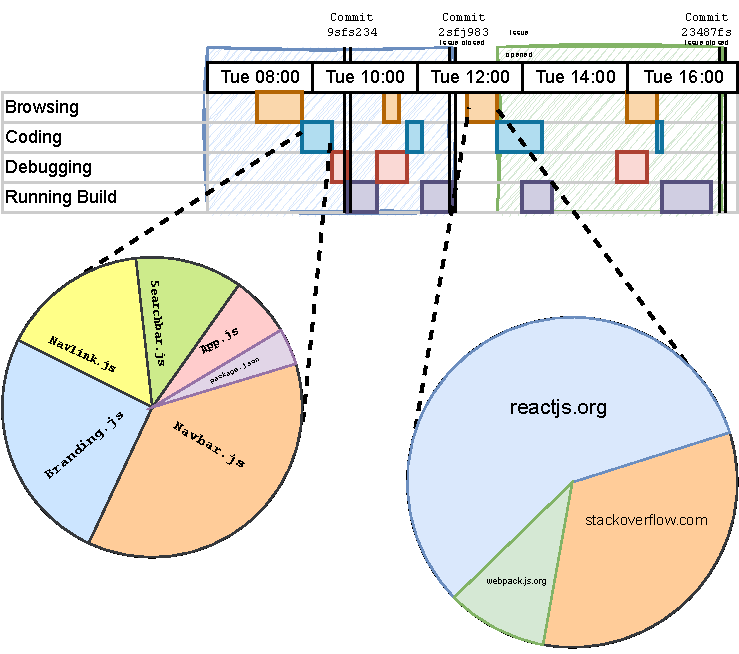
\includegraphics[width=0.4\textwidth]{sampleviz.pdf}
    \caption{Example of efforts spent on a timeline}
\end{figure}

%====================================================
\section{Programme and methodology}

% Detail and justify the research methodology.

% Describe the work programme including research and impact-related activities to be undertaken.

% Identify the contribution of each member of the research team including any project partners and stakeholders.

% Provide objectives and milestones that will be used to monitor progress and explain how the project will be managed.

To attain the provided objectives, the approach outlined would monitor progress \& explain how the project will be managed over milestones while detailing the methods \& techniques for conducting the research with successful outcomes.

\subsection*{Initial Research (WP1)}

The project will begin by undertaking background research including surveying the knowledge with published papers in the area of developer experience \& task estimations through a literature review, investigating current existing solutions, and determining the intended audience for the project evaluation; this would help us inform the design \& development of our study. We expect to run our background survey for six months.

\textbf{Literature:} There are many aspects to development processes and experiences since it involves human factors, and to understand developers, we will conduct a comprehensive literature review to identify the key areas of research related to our topic, including \textit{developer productivity}, \textit{developer learning}, \textit{software practices}, \textit{team structures}, and \textit{industry experience}. Extracting published knowledge from these fields could provide more context, to realise the current state of research and identify gaps, than surveying papers solely on the lower amount of papers specifically on Developer Experience.

\textbf{Current Solutions:} The proposed tool should provide a unique solution to the research problem of developer frustrations with project management \& task estimations, and it is important to investigate existing services that provide solutions, acknowledging their efforts. See \autoref{existingSolutions} for examples. In surveying and understanding their dashboards, we could also outline the requirements of our application in terms of features and functionality with potential opportunities for innovation.

\begin{figure}[h]
    \centering
    \begin{subfigure}[b]{0.1\textwidth}
        \centering
        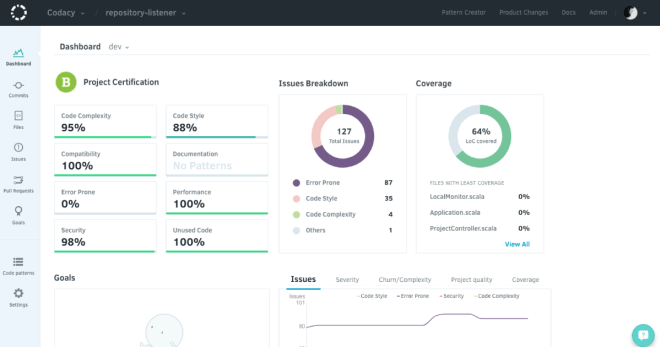
\includegraphics[width=\textwidth]{codacy_dashboard.png}
        \caption*{{\footnotesize Codacy}}
    \end{subfigure}
    \hfill
    \begin{subfigure}[b]{0.1\textwidth}  
        \centering 
        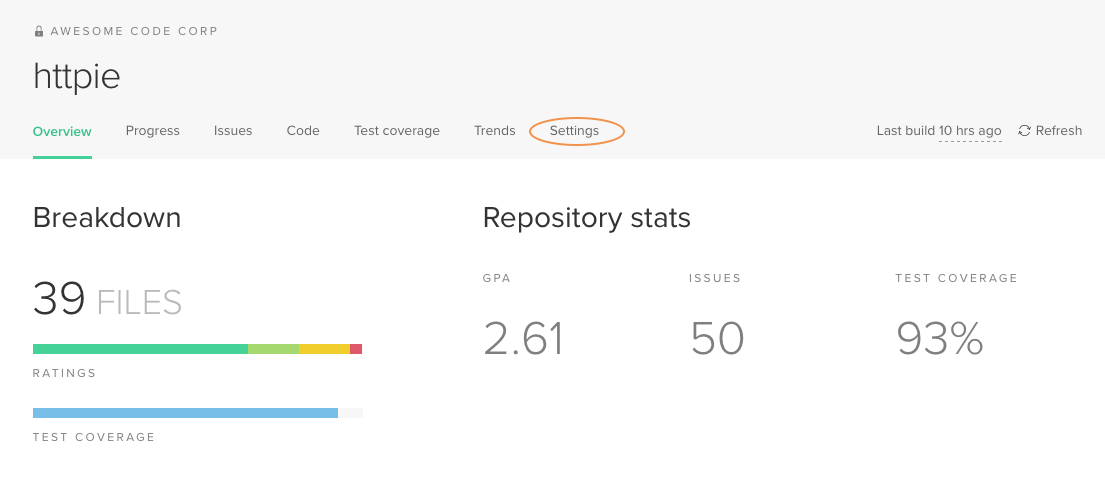
\includegraphics[width=\textwidth]{codeclimate_dashboard.png}
        \caption*{{\footnotesize CodeClimate}}
    \end{subfigure}
    \hfill
    \begin{subfigure}[b]{0.1\textwidth}   
        \centering 
        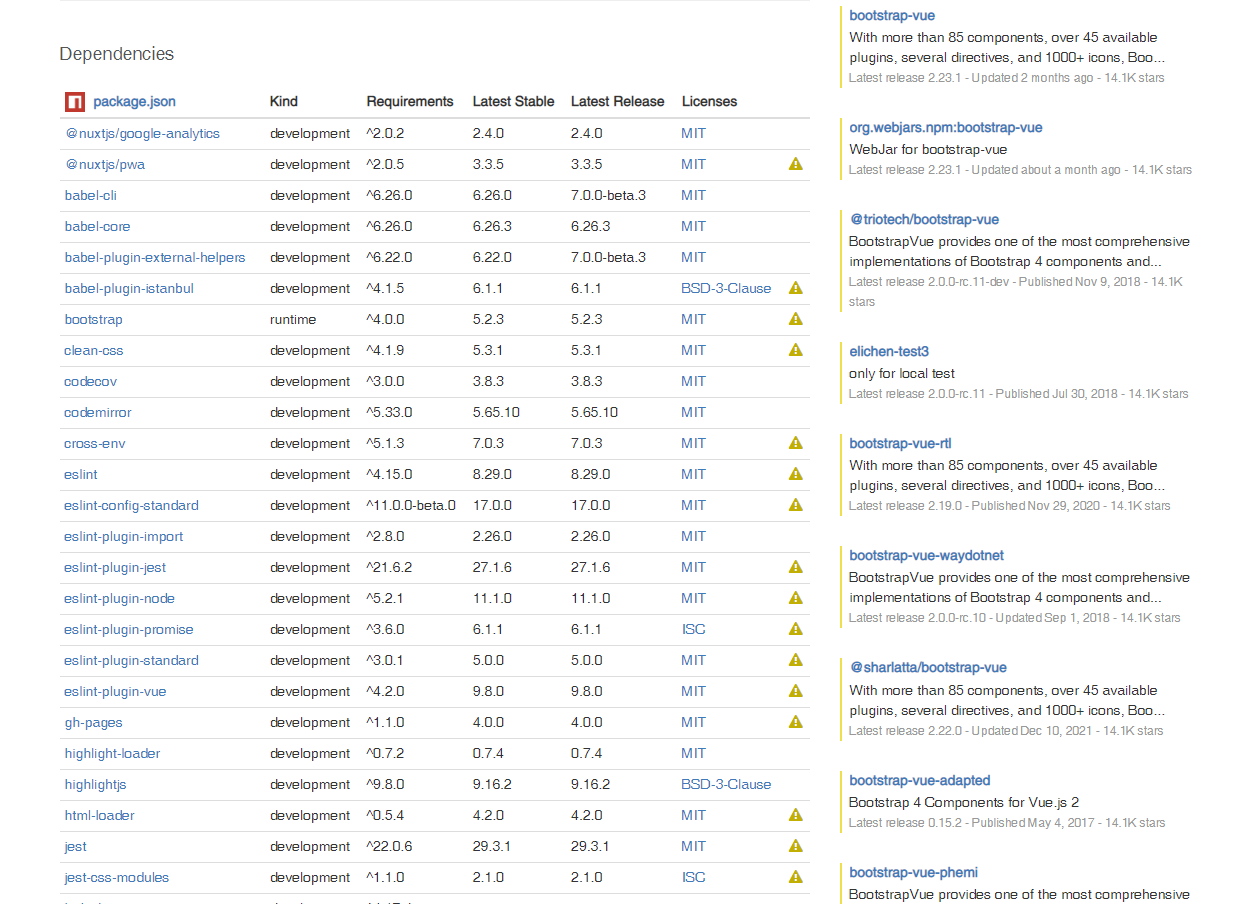
\includegraphics[width=\textwidth]{librariesio_dashboard.png}
        \caption*{{\footnotesize Libraries.io}}
    \end{subfigure}
    \hfill
    \begin{subfigure}[b]{0.1\textwidth}   
        \centering 
        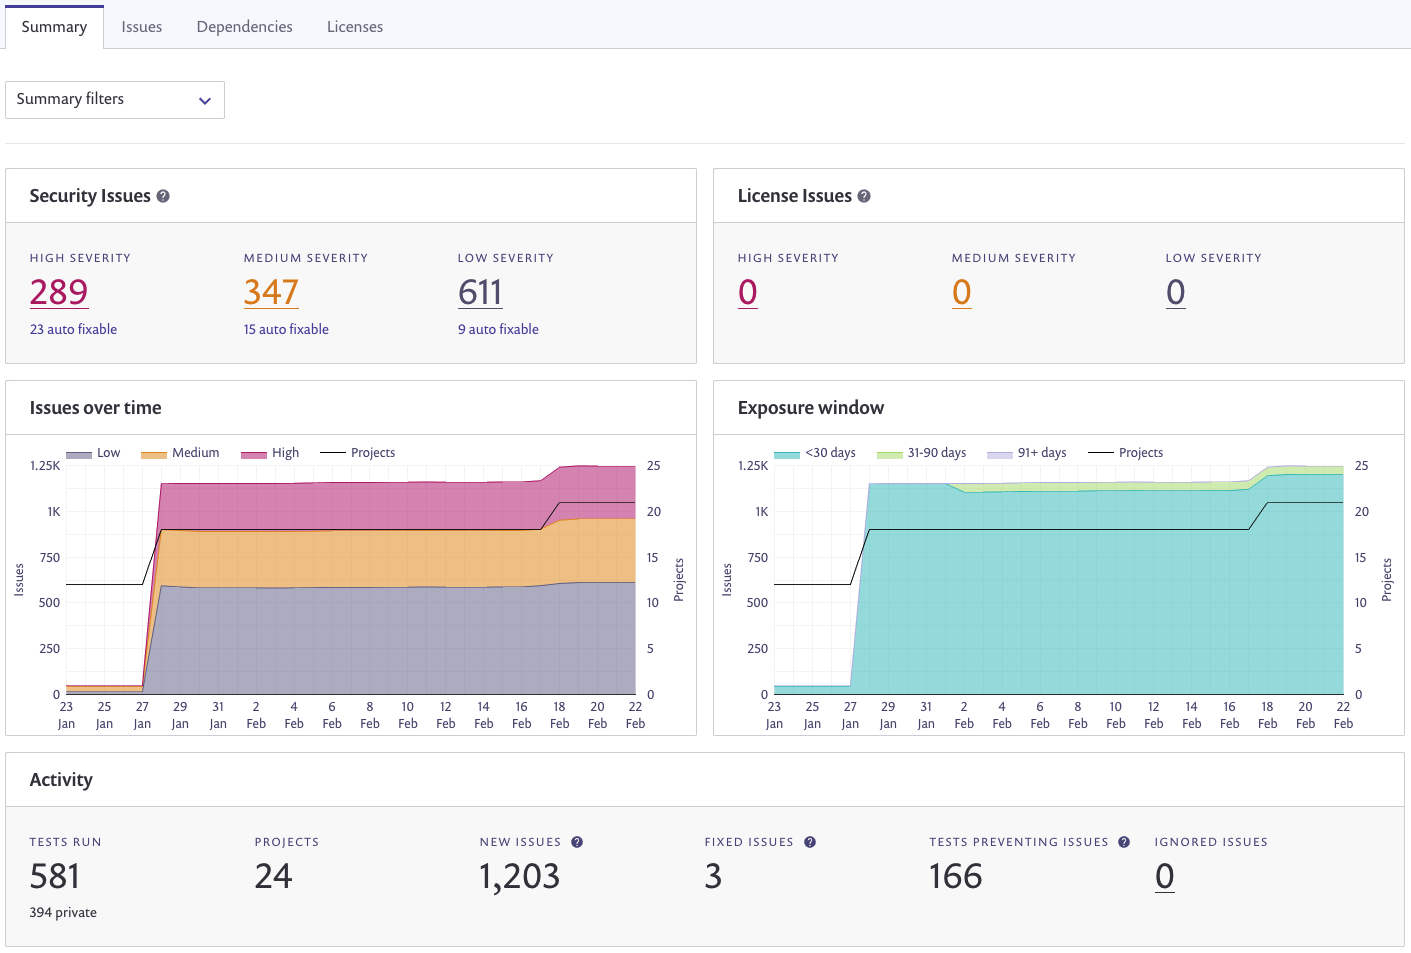
\includegraphics[width=\textwidth]{snyk_dashboard.png}
        \caption*{{\footnotesize Snyk}}
    \end{subfigure}
    \caption{Dashboards for different code monitoring services}\label{existingSolutions}
\end{figure}

\textbf{Audience:} Developing the application would benefit from knowing the end-users. Through observations and interviews with developers, we will understand their workflow \& project management structure and also scope the participants for the evaluation of the project. This includes having discussions with developers in relatively close physical proximity to the project location (Glasgow, UK) that agree to share their thoughts on their development activity, along with studying workflows of popular open-source repositories on GitHub that formally use issue management with discussion threads.

\subsection*{Application Implementation (WP2)}

After conducting initial research and scoping the requirements of our tool, we move to the implementation process including designing the dashboard and engineering the architecture.

\begin{figure}[h]
    \centering
    \begin{subfigure}[b]{0.08\textwidth}
        \centering
        
\includegraphics[width=\textwidth]{vscode_logo.png}
        \caption*{{\footnotesize VSCode}}    
    \end{subfigure}
    \hfill
    \begin{subfigure}[b]{0.075\textwidth}
          \centering
          \begin{overpic}[width=0.9\textwidth]{svelte_logo.png}
             \put(50,5){
\includegraphics[width=0.5\textwidth]{vite_logo.png}}  
          \end{overpic}
        \caption*{{\footnotesize SvelteKit}}
    \end{subfigure}
    \hfill
    \begin{subfigure}[b]{0.08\textwidth}
        \centering
        
\includegraphics[width=\textwidth]{chartjs_logo.png}
        \caption*{{\footnotesize Chart.js}}
    \end{subfigure}
    \hfill
    \begin{subfigure}[b]{0.08\textwidth}  
        \centering 
        
\includegraphics[width=\textwidth]{github_logo.png}
        \caption*{{\footnotesize GitHub}}    
    \end{subfigure}
    \hfill
    \begin{subfigure}[b]{0.08\textwidth}  
        \centering 
        
\includegraphics[width=\textwidth]{wakatime_logo.png}
        \caption*{{\footnotesize WakaTime}}    
    \end{subfigure}
    \caption{Core technologies for the application}
\end{figure}

We target to implement this on a public repository over a year with our team of experienced developers. The application would involve interactions with multiple APIs, each with restrictions such as authorisation and rate limits, integrating into each other at the right time without adding to the mental load of the developers -- facilitating these moving parts of the system while providing modularity would be a huge task and so planning the system architecture with the initially chosen tools is essential. A Visual Studio Code\cmmnt{\cite{VisualStudioCode}} extension built using SvelteKit\cmmnt{\cite{SvelteKitWebDevelopment}} and Chart.js\cmmnt{\cite{ChartJs}} would provide opportunities for scaling the project with easy development due to their popularity and the API they offer. The initial plugins for Software as a Service (SaaS) platforms would be GitHub and WakaTime.

\begin{figure}[h]
    \centering
    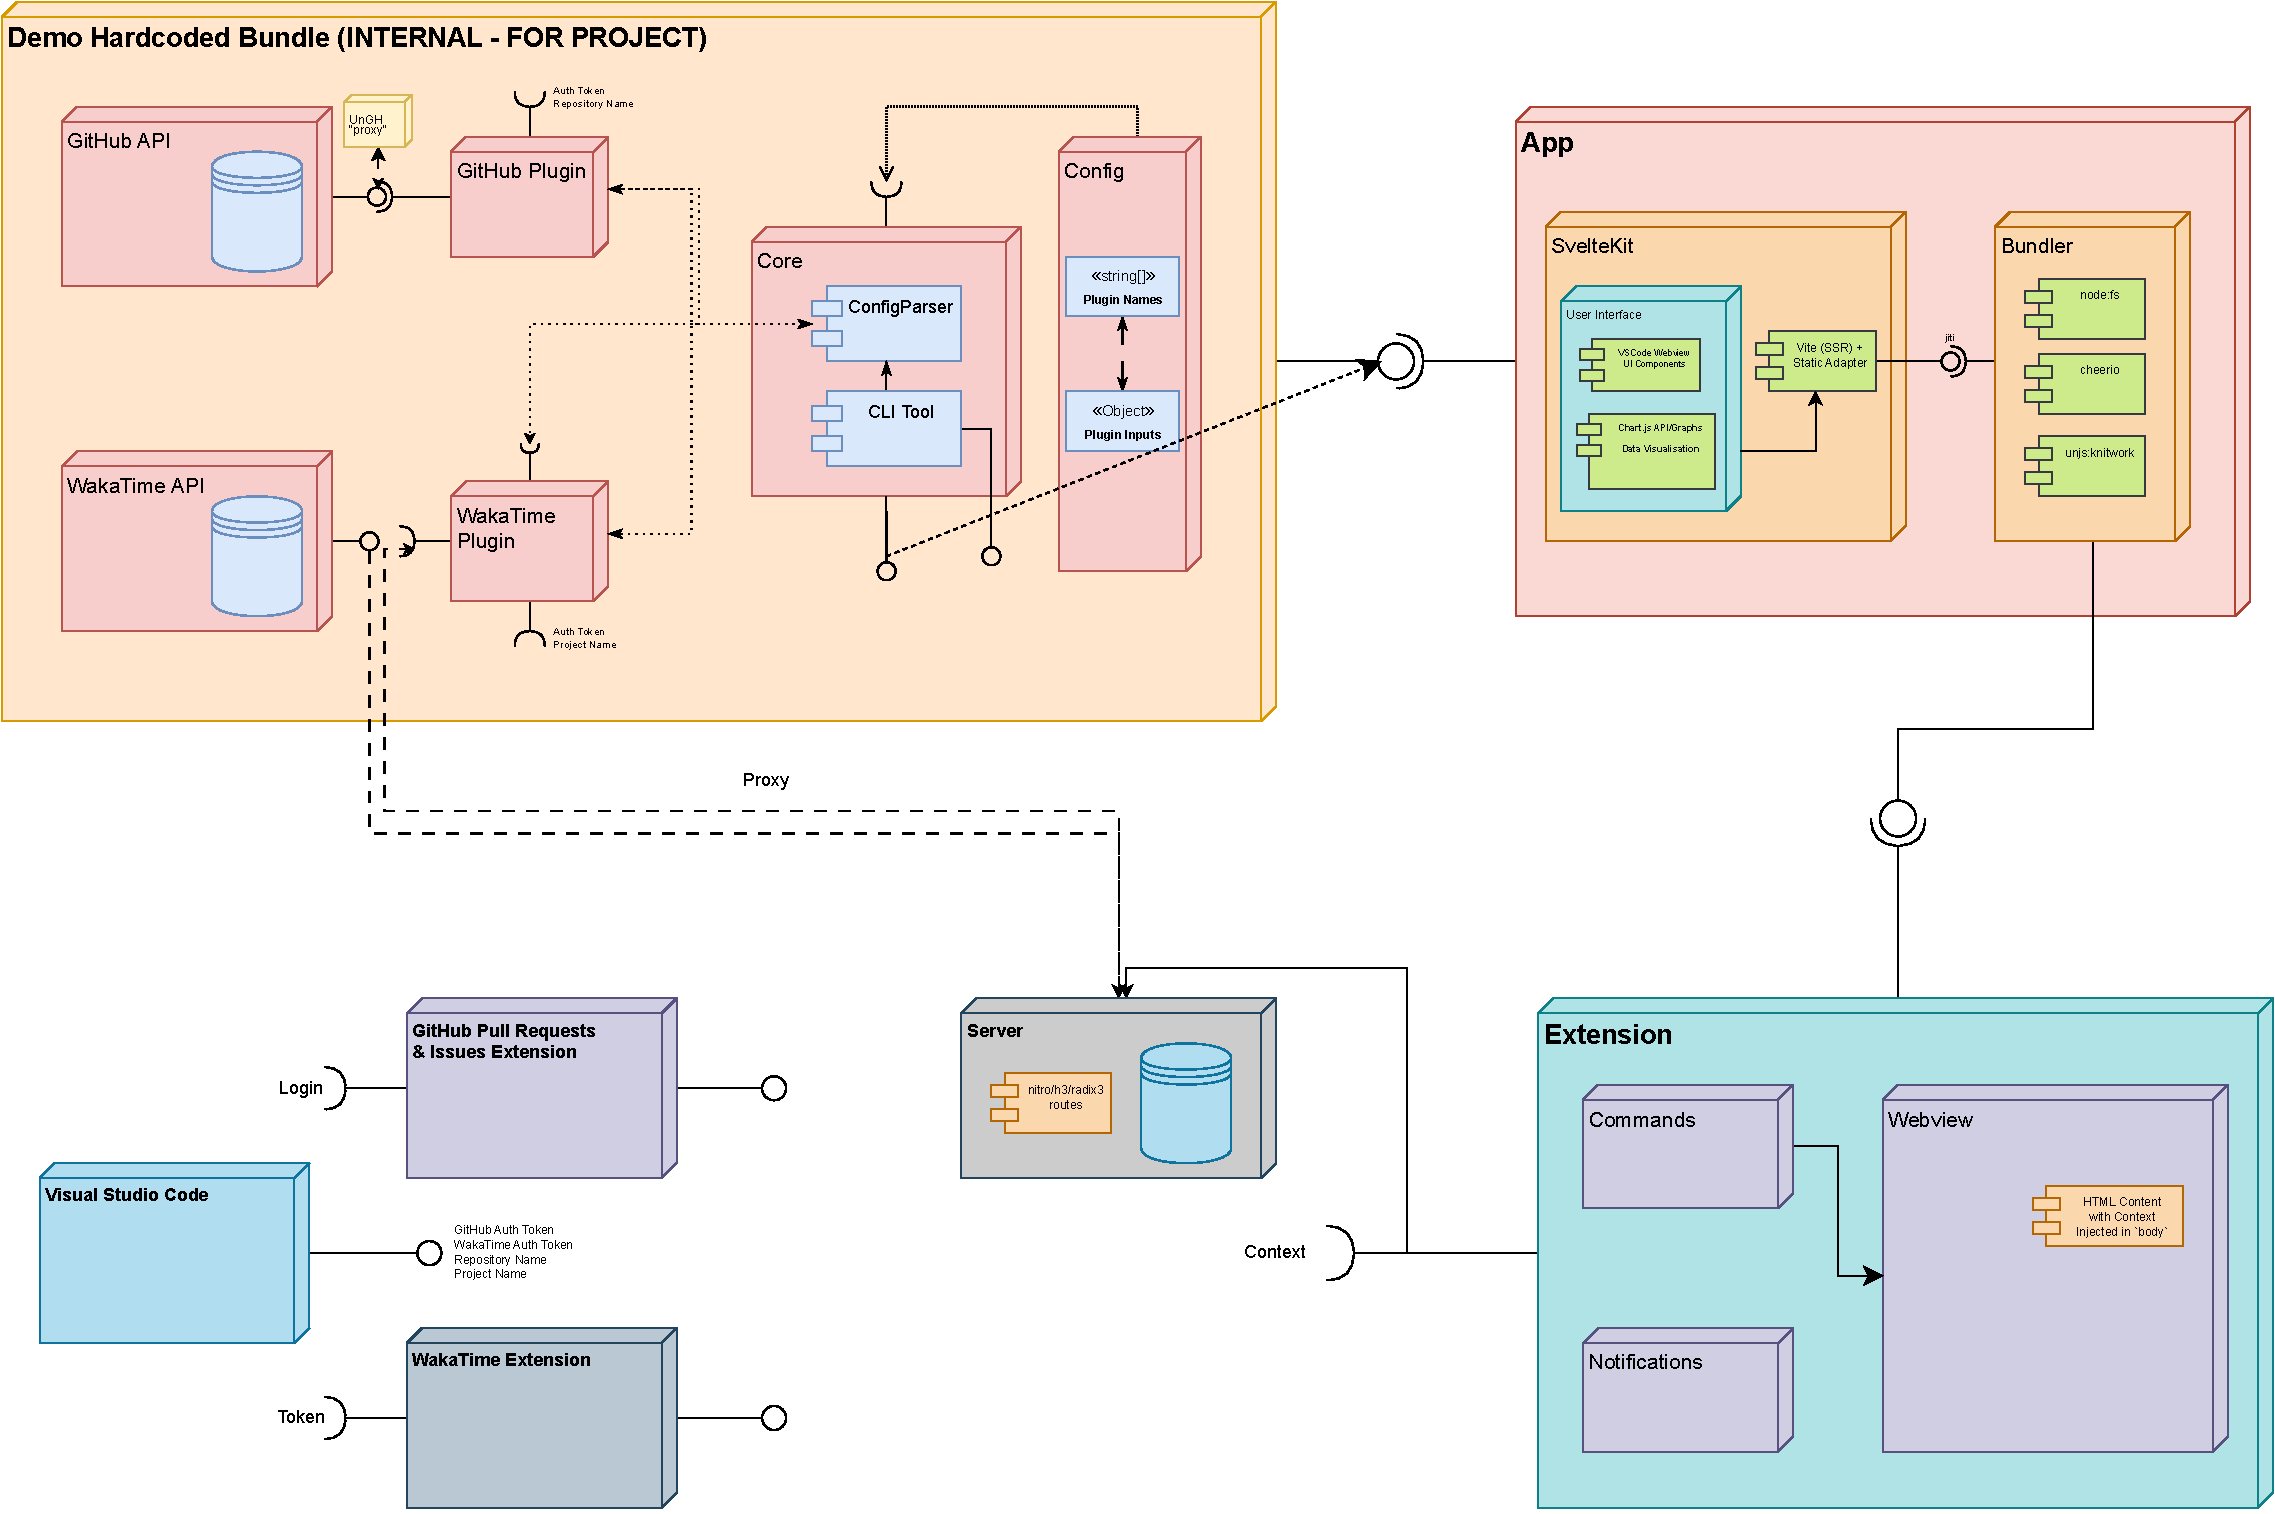
\includegraphics[width=0.45\textwidth]{architecture.pdf}
    \caption{Planned architecture for the tool}
\end{figure}

\textbf{VSCode Webview:} The Visual Studio Code Webview API allows extensions to create fully customisable views within the editor\cmmnt{\cite{WebviewAPI}} since it is built using Electron that renders Chromium browser instances for cross-platform applications, so web-apps using HTML, CSS \& JavaScript can be added to it\cmmnt{ (we would adhere to the VSCode UI)}; however, the environment is not the same as a traditional web-browser, so the restrictions would need to be considered. Moreover, even though there are other options like the sidebar and popups, the main panel that is used to view \& edit code, (also provides tabbed headings to multiple panels) would be ideal for our dashboard to display large graphs.

\begin{figure}[h]
    \centering
    \begin{subfigure}[b]{0.22\textwidth}
        \centering
        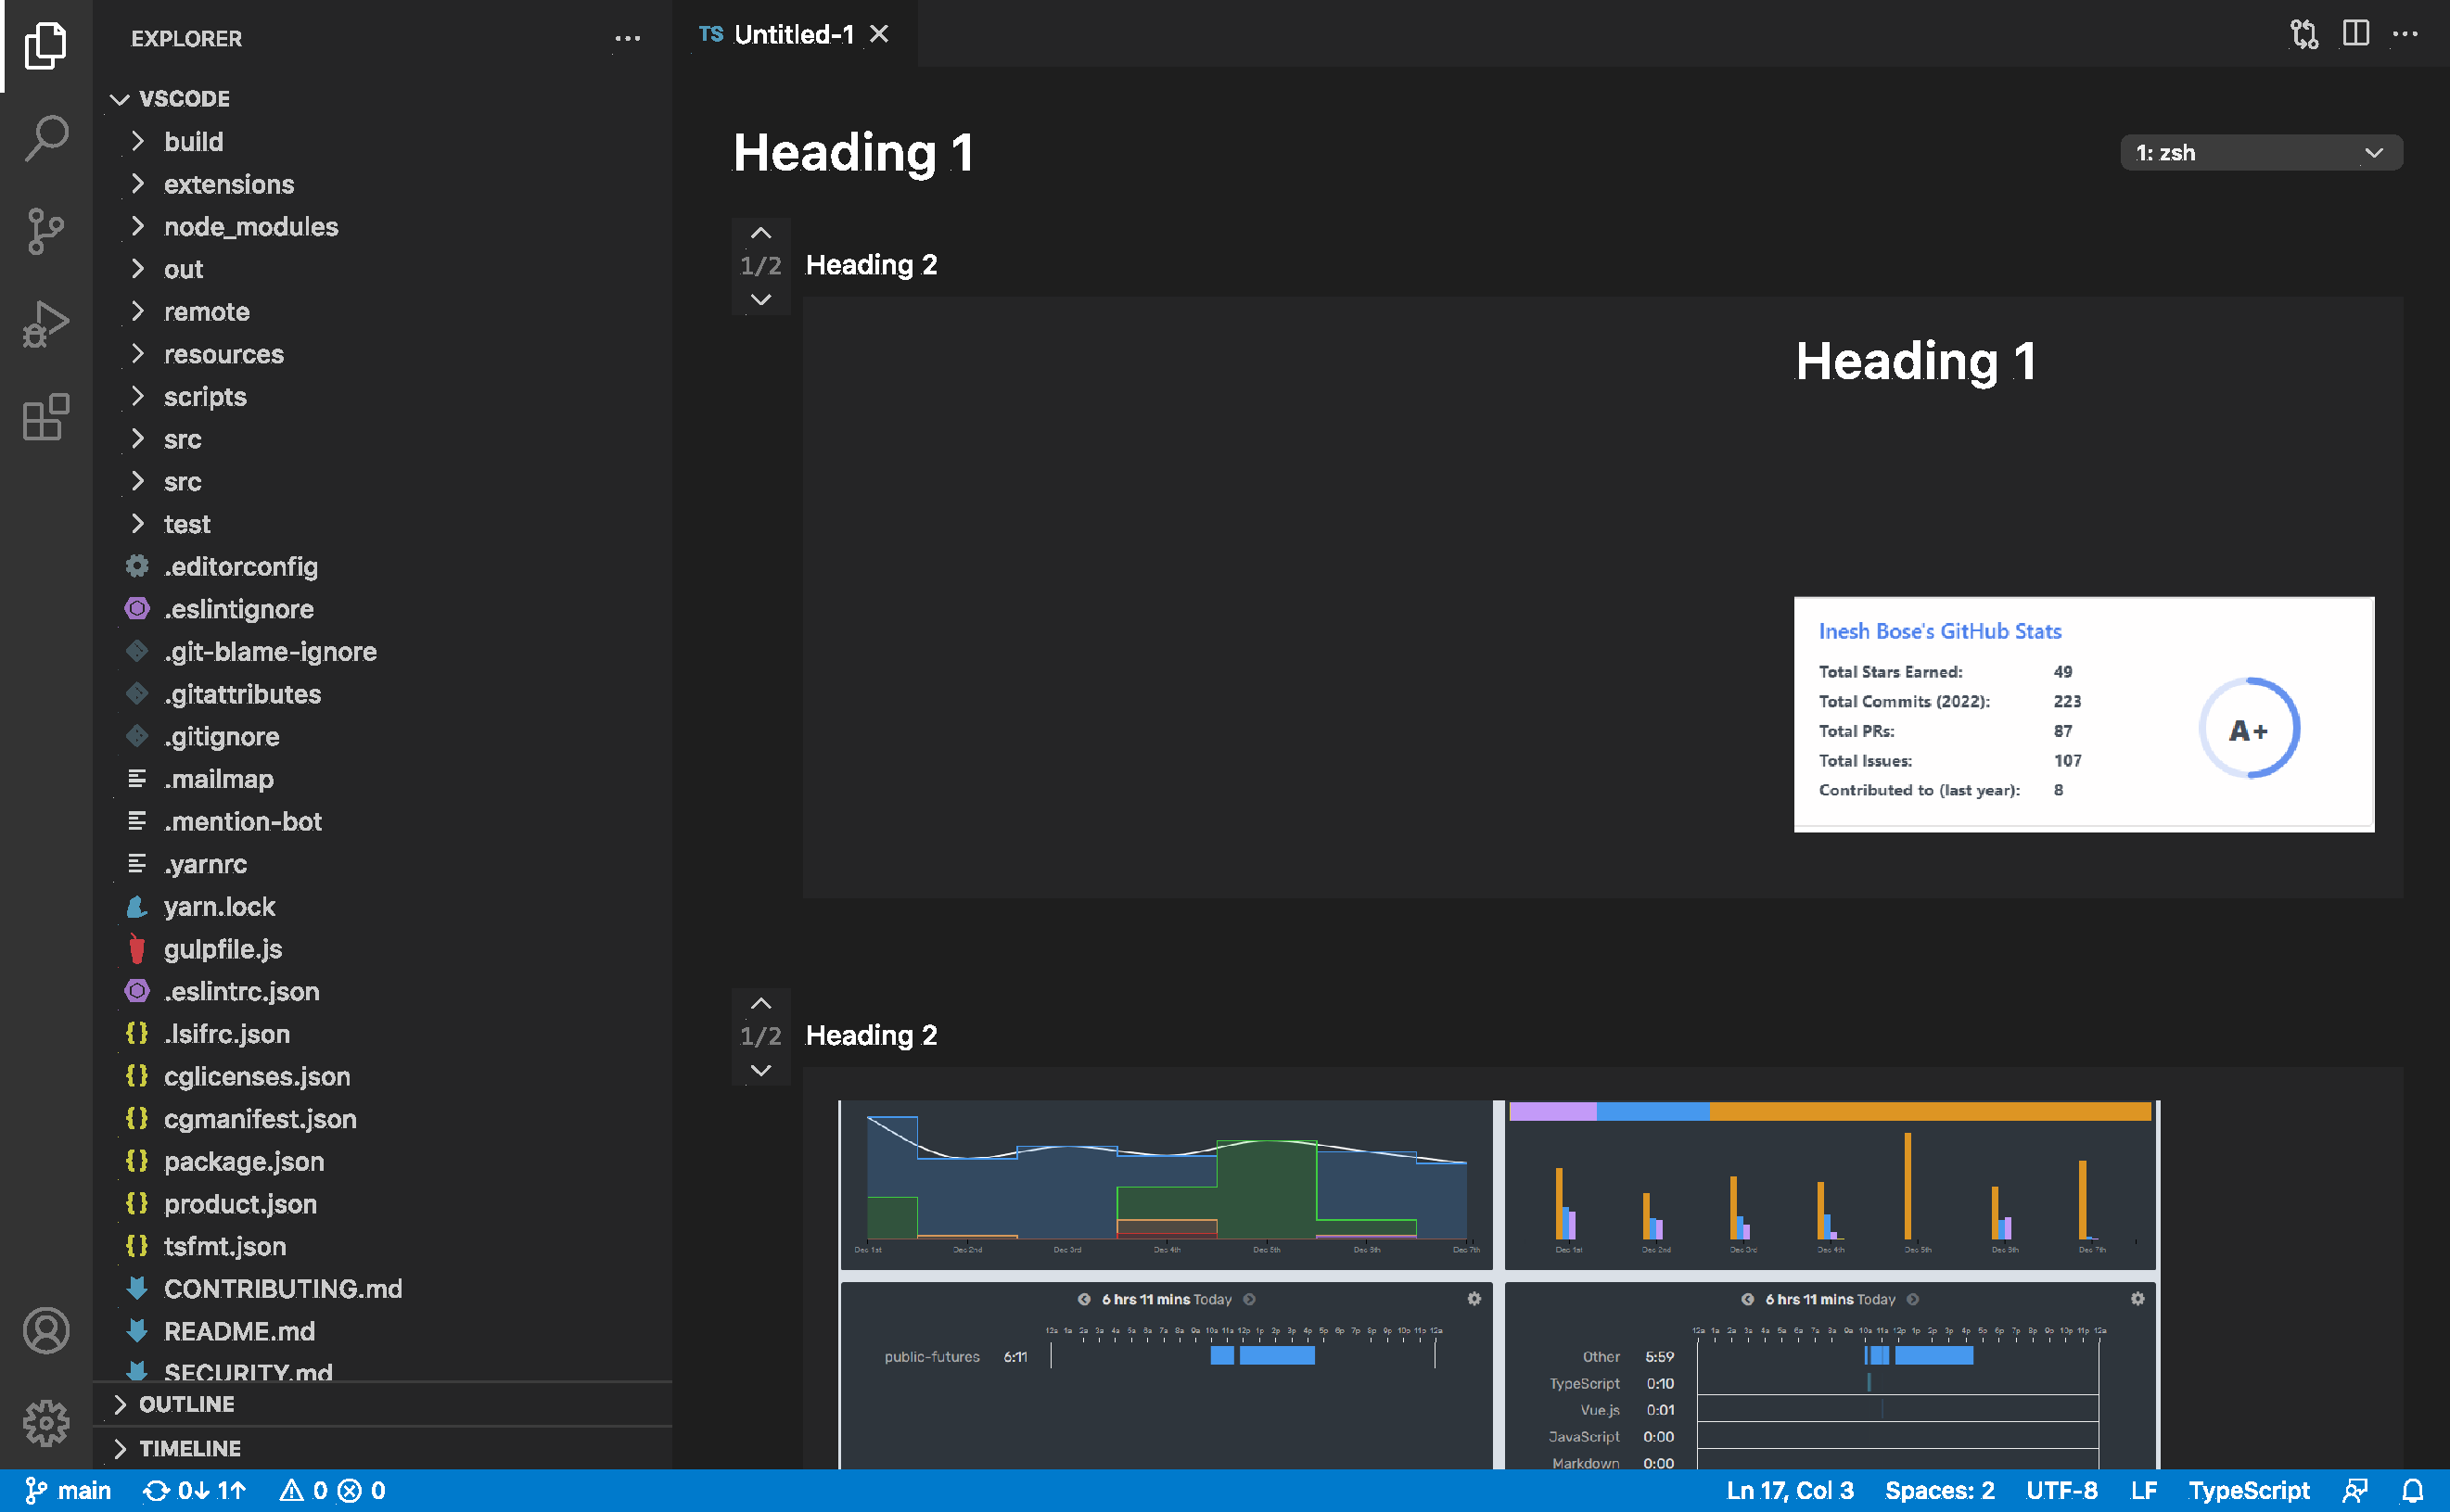
\includegraphics[width=\textwidth]{initialwf.pdf}
        \caption*{{\footnotesize Initial Wireframe}}
    \end{subfigure}
    \hfill
    \begin{subfigure}[b]{0.25\textwidth}  
        \centering 
        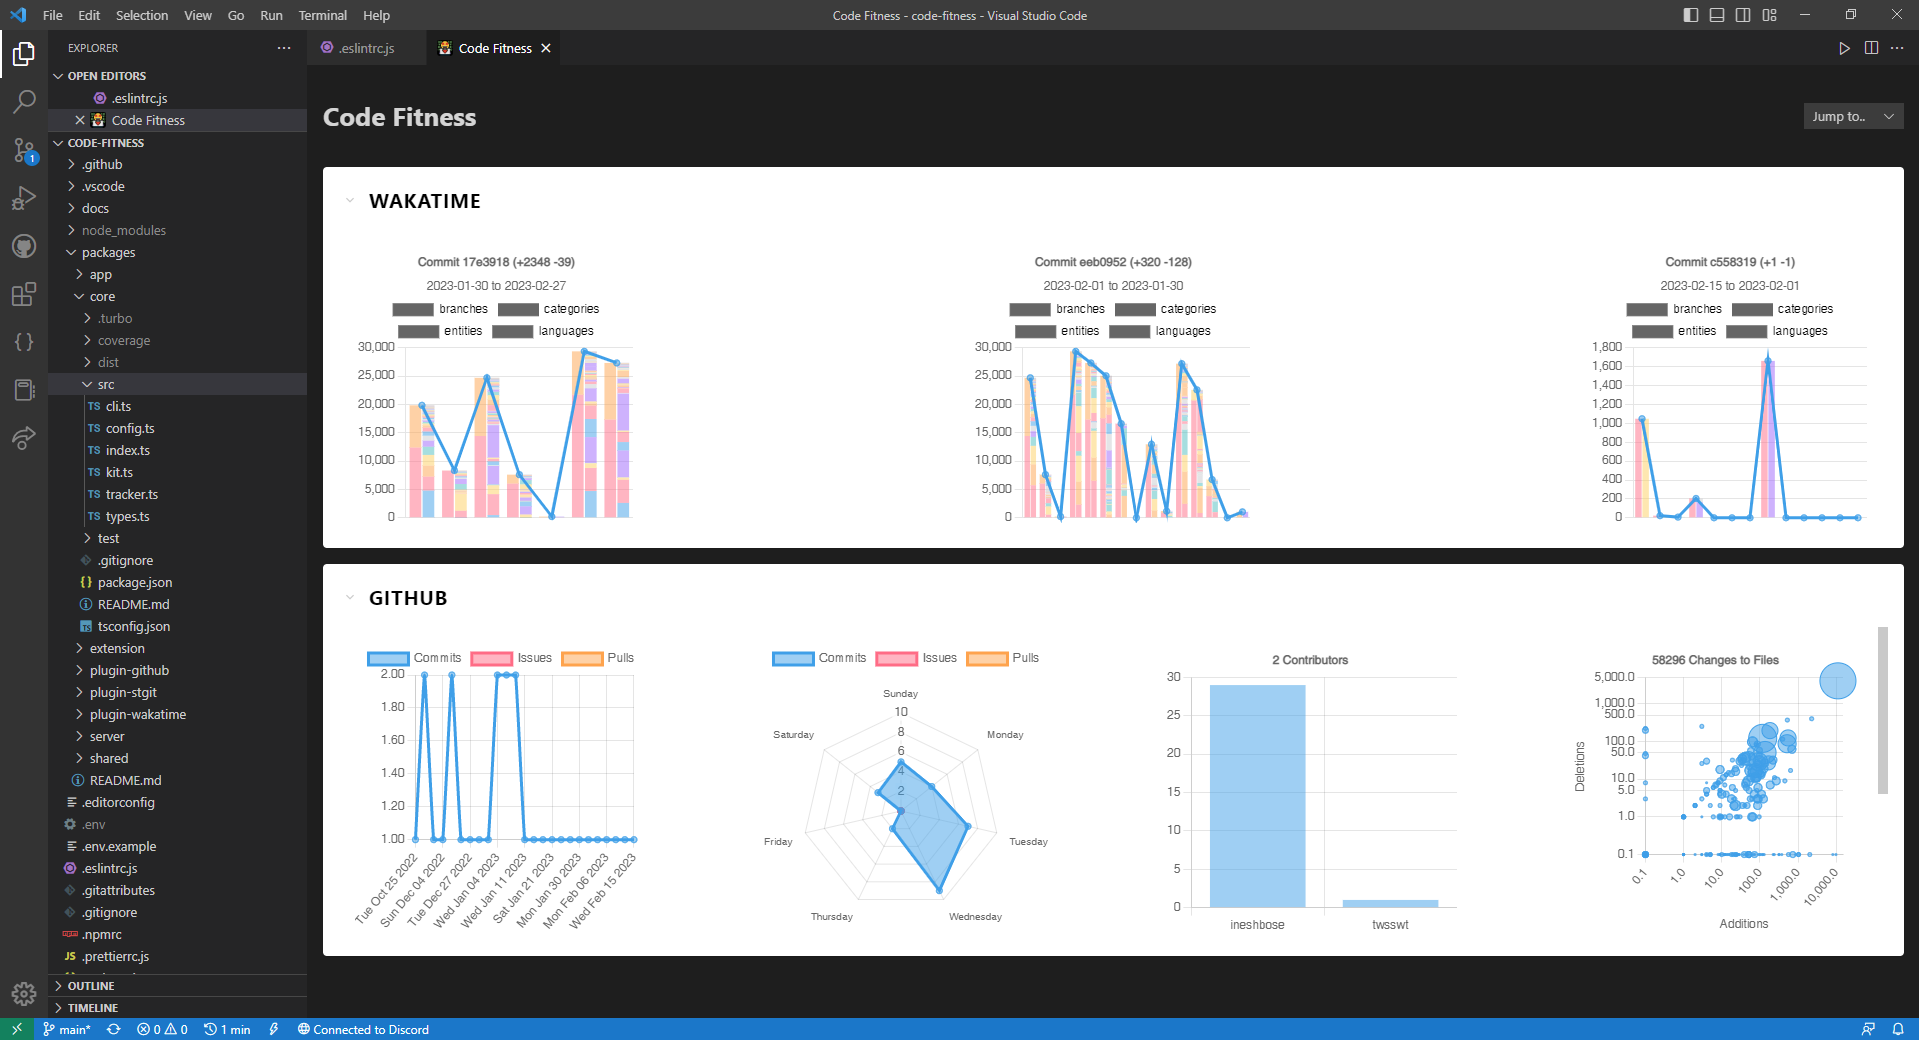
\includegraphics[width=\textwidth]{screenshot_27-02.png}
        \caption*{{\footnotesize Implemented (so far)}}
    \end{subfigure}
    \caption{Progress on the Dashboard UI Design} 
\end{figure}

\textbf{SvelteKit:} SvelteKit is \cmmnt{a language \cmmnt{\cite{262588213843476TruthSvelte}} and }a frontend framework written in TypeScript (typed, syntax superset JavaScript)\cmmnt{\cite{harrisSvelteRethinkingReactivity2019}} using single-file components written in Svelte to render UI on the DOM (Document Object Model; rather than Virtual-DOM)\cmmnt{\cite{harrisVirtualDOMPure2018}}, and it is one of the most loved frameworks \cite{StateJS2021}. While it is relatively new, we aim to use DX-focused tools to serve a high-performance static single-page application (SPA) with the ability to use additional functionalities, such as built-in file-based routing and server-side rendering, when required. VSCode provides a frame within webviews and extensions are TypeScript-focused ensuring bug-free development; Svelte enables us to take advantage of these. Moreover, SvelteKit uses Vite for facilitating extremely fast development and builds, and to avoid caching issues, Vite uses file-hashing causing filenames in builds to be unique and unpredictable (this is intended and good for the system). Since VSCode Webview expects HTML templates to be provided as a string, an additional bundle adapter would be designed to keep builds compatible \& easy to maintain.

\textbf{Chart.js:} Generating graphs on websites requires \texttt{canvas} elements and JavaScript that may need a great amount of logic to be abstracted for unknown data. Instead, Chart.js is an established, open-source community maintained project, with over 2M downloads weekly downloads, providing different charts with great performance, responsiveness and customisation. Rendering a graph only requires a JSON object to be passed, and with the usage of TypeScript, we can declare a schema of input ensuring the consistency of the data.

\textbf{GitHub Plugin:} With more than 100 million users, the majority of remote repositories are hosted on GitHub. With a powerful and well-documented API, we need to leverage it to get data about their project and changes over the commit history. However, we expect some of our target participants to use different services such as a private, self-hosted instance of GitLab; that would need a different plugin but with similar logic.

\textbf{WakaTime Plugin:} WakaTime provides a solution close to our project; it is a software productivity analytics service that collects and displays developers' coding activities through a range of integrations and plugins for popular development environments in addition to an API. This is extremely useful to the project and would remove massive complexities required for our implementation; the application would map the data from the WakaTime API to the repository data from their hosting service and display suitable, intuitive graphs.

\textbf{Deployment:} The final step for wrapping up the development of the application would be to publish it on a platform that users and participants can easily access. Ensuring that no bugs are experienced with the VSIX build in different environments and setups, it would get added on Visual Studio Marketplace.

\subsection*{Participant Recruiting (WP3)}

The evaluation of the application is required to be conducted with developers i.e. people that have knowledge of software development and are involved in a process. Based on this knowledge and their level of experience, we will recruit developers in cohorts over a period of four months\cmmnt{ to ensure a good participant sample}.

\textbf{The Beginner:} Participants that are new to issue management and task estimations may not see the benefits of the dashboard immediately due to their limited experience, but it would be helpful to introduce the dashboard's concepts from them while gaining feedback from a novice's point-of-view.

\textbf{The Intermediate:} Developers that have had some experience with the topic area by working on projects requiring issue management are the main target audience and hence the core participant cohort. As they work on their projects over sprints \& iterations, the metrics from the dashboard could pose to be more useful to them and help improve task estimation for future milestones; this is what we want to record.

\textbf{The Experienced:} These developers would have significant experience using issue management as part of their workflow and being used \& required in projects they work on. Collecting their feedback and expertise on the dashboard would greatly help the research in software metrics and dashboard designs.

\subsection*{Evaluation (WP4-6)}

The process for evaluating the project aims to assess the effectiveness of our dashboard. Given the structure of data collection required by the application and iterative development of software, the study should fit into the developers' process and be carried out as a longitudinal study over a year.

\textbf{Introduction \& Setup:} After recruitment to participate in the study, for the beginning of the evaluation, developers would be provided with an overview of the dashboard and also be assisted in getting setup with the extension on their personal devices they use for development for the next few weeks. Participants can optionally provide demographic information in their consent form; this would help in understanding any biases.

\textbf{Weekly Feedback:} As the participants work on their software projects and there is more data available to display on the charts, we would ask them to provide feedback on their experience using the dashboard in weekly checkpoints. The feedback form would ask them to describe their week of working on their projects, if the dashboard had an effect on their week if there were metrics they were not expecting, and if they had any bug fixes or feature requests to report.

\textbf{Retrospective:} At the end of the evaluation period, we will conduct a retrospective meeting, where we will study the dashboard with the data collected over the weeks and gather in-depth feedback from the participants on their overall experience with the dashboard. This will wrap up the evaluation.

\subsection*{Analysis (WP7)}

The final work plan involves analysing the data collected from the evaluation and testing them to confirm if the research objectives were successful. Since the data is qualitative, it would be transformed into information that can be used to identify patterns and trends in the developers' weekly feedback. We aim to have an outcome after six months of analysis.

\textbf{Preparing:} Survey data would be collected from online forms and exported into a spreadsheet, and feedback collected through interviews \& focus groups (during the retrospective meetings) would be transcribed into text format.

\textbf{Coding:} After reading and understanding the data, any themes, based on the dashboard implementation, that emerge from the feedback would be identified also helping in further categorising data in groups. This would also be aided by qualitative analysis software such as NVivo and Atlas.ti.

\textbf{Interpretation:} Judging from the common themes and patterns in the data, we can interpret the results to make recommendations for the tool and/or create our conclusion.

%====================================================
\section{Impact of the project}

% Impact is a core consideration throughout the grant application process. Showing how you will maximise the impact of the proposed research should therefore be intrinsic to the proposal itself in a way that is appropriate to the nature and scope of the research being proposed.

% For example, in proposals focused on discovery research the proposal may focus principally on the generation of new knowledge, whilst proposals with significant elements of applied research may have impacts related to economic and societal benefits.

Maximising the impact of the proposed research is a critical consideration in this project. The shared knowledge from our literature survey and our application showing how a centralised dashboard can affect developer experience and the potential for future resource allocation enables great impacts.

\subsection*{Academic Impact}

This research will contribute to the academic community's understanding of developer experience, which is a relatively new research field. By providing empirical evidence on the effectiveness of the dashboard, this research can help identify areas of improvement in the development process, and given the modular architecture, it will provide a framework for other researchers to build upon, helping to create an ecosystem and advance the understanding of developer experience.

\subsection*{Practical Impact}

Developers, both indie and in companies, can use the outputs of this project to realise resource allocation, leading to potential economic and societal benefits. By providing developers with a highly customisable dashboard with relevant metrics, it can enable them to make informed decisions about their development process and avoid technical debt leading to more efficient \& effective software. Companies and organisations can use our findings and tool (also for creating plugins) to understand the importance of providing developers with suitable tools that enhance their experience, therefore allowing productivity, job satisfaction and employee retention to increase.

\let\oldbibliography\thebibliography
\renewcommand{\thebibliography}[1]{\oldbibliography{#1}
\setlength{\itemsep}{-3pt}}

% \bibliographystyle{abbrv}
%\setstretch{0.8}
{
\renewcommand*{\bibfont}{\scriptsize}
\printbibliography
% \printbibliography[notcategory=cited,heading=subbibliography,title={Further Reading}]
}
\end{document}
